\chapter{Context-aware and recommender systems}
\label{cha:recommenders}

Both topics---context-aware systems and recommender systems---have been growing more and more popular among researchers lately. Both can be discerned to have approximately equivalent curves on accumulated paper and citation counts in time, as shown in \cref{fig:scholar-context-aware} and \cref{fig:scholar-recommender-systems}. Result were obtained after processing 8098 and 3420 papers, respectively, that is all papers that have been found for ``recommender systems'' and ``context-aware'' queries in Google Scholar and Microsoft Academic Search. The S-like shape of the curves might suggest that the topic has already been researched thoroughly.

\begin{figure}
	\centering
	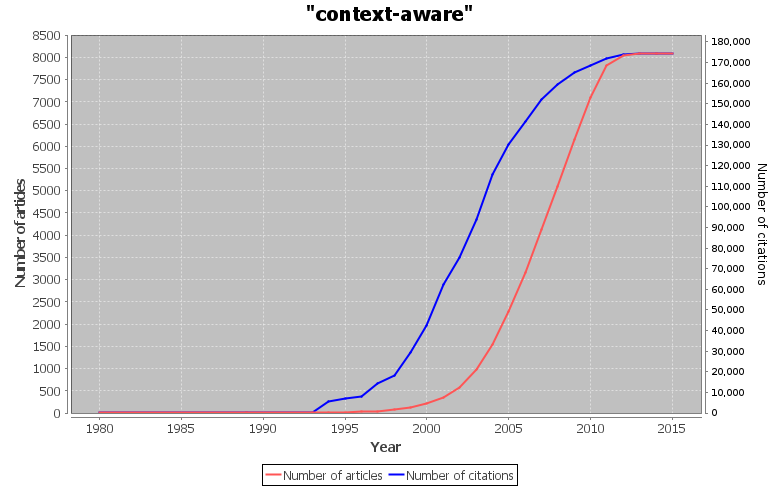
\includegraphics[width=\textwidth]{scholar-context-aware}
	\caption{Google Scholar and Microsoft Academic Search accumulated trending for ``context-aware'' query \cite{Rus:scholar-trends}.}
	\label{fig:scholar-context-aware}
\end{figure}

\begin{figure}
	\centering
	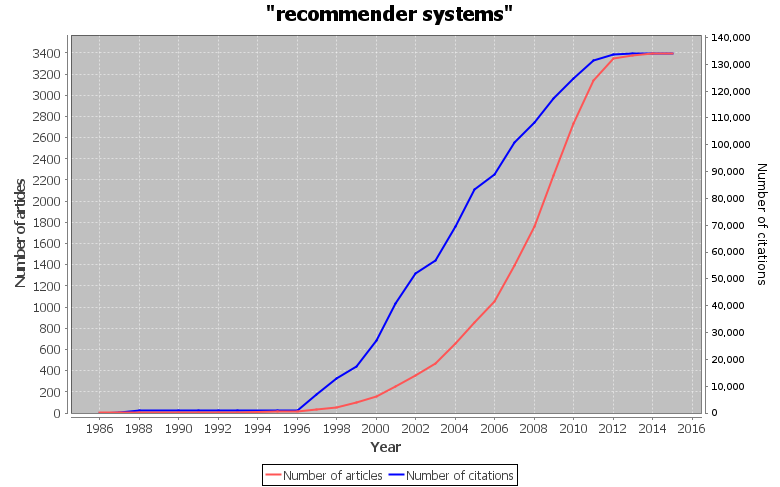
\includegraphics[width=\textwidth]{scholar-recommender-systems}
	\caption{Google Scholar and Microsoft Academic Search accumulated trending for ``recommender systems'' query \cite{Rus:scholar-trends}.}
	\label{fig:scholar-recommender-systems}
\end{figure}

\section{Context-aware systems}

The term, context-awareness, refers to the ability of the system to sense/be aware of its environment. This term mainly applies to mobile systems which are more likely to have their surroundings changed frequently. It is in a way similar to location awareness but expands beyond just location. Various researchers identify different elements of the context, e.g.:

\begin{itemize}
	\item user, role, identity \cite{Dey:context} \cite{Kaltz:context},
	\item process, task \cite{Kaltz:context},
	\item location \cite{Dey:context} \cite{Kaltz:context},
	\item time \cite{Dey:context} \cite{Kaltz:context},
	\item device \cite{Kaltz:context},
	\item activity \cite{Dey:context},
	\item nearby people and devices \cite{Rosslin:context},
	\item lighting and noise level \cite{Rosslin:context},
	\item network availability \cite{Rosslin:context},
	\item even the social situation (relations between the user and their peers nearby) \cite{Rosslin:context}.
\end{itemize}

By keeping track of this variables over the period of time, a system that would be classified as a context-aware one, could infer things that would be useful to the user. These might include turning on appropriate application on a mobile device when a certain set of conditions is met etc.

Context awareness is also an important concept in so called ubiquitous computing or just \emph{ubicomp}. To the regular user, ubicomp---also called pervasive computing and, more recently and commercially, Internet of Things---appears as if the computing processes were happening literally anywhere between a large network of distributed devices. These small, inexpensive devices equipped with various sensors share information among themselves as well as with services run by manufacturers, in order to provide the end user with some greater value.

Some exemplary use cases for a ubiquitous system might include:

\begin{itemize}
	\item ``domestic ubiquitous computing environment might interconnect lighting and environmental controls with personal biometric monitors woven into clothing so that illumination and heating conditions in a room might be modulated, continuously and imperceptibly'' \cite{wiki:ubiquitous},
	\item ``refrigerators «aware» of their suitably tagged contents, able to both plan a variety of menus from the food actually on hand, and warn users of stale or spoiled food'' \cite{wiki:ubiquitous}.
\end{itemize}

Thus, it is safe to say that ubiquitous computing would not be able to function without context-awareness.

An interesting research that is taking place in recent years, and is definitely worth taking a closer look at, concerns data gathered by the AWARE Framework.

AWARE Framework is an application and a library with a main purpose of gathering mobile context information. Analyzed sensors include: accelerometer, barometer, battery, running applications, Bluetooth, communication activities, gravity, gyroscope, locations, the level of light, network connectivity, temperature and many more. \cite{aware}

The collected data is sent to a pre-configured web service running a SQL data base in the back-end, where it can afterwards be analyzed by researchers. Furthermore it provides non-academic developers to enhance User Experience of their applications. By using the context information, they are able to plan notification/interruption moments more sanely. \cite{aware}

Choosing which elements of context are relevant for a given case is quite demanding, as there are many points to take into consideration. As AWARE developers put it, ``Capturing context is challenging. In fact, context is produced anytime, anywhere, by everything and anyone: it is extremely volatile and subjective.'' \cite{aware} One also has to think of such a mundane question as\ldots battery life of the mobile device.

\vspace{4cm}
\todo{Cite something by S. Bobek}

\clearpage

\section{Recommender systems}